\documentclass[midd]{thesis}

\usepackage{graphicx}
\usepackage{times}
\usepackage{url}
\usepackage{listings}

\lstset{basicstyle=\ttfamily\footnotesize,breaklines=true}

\graphicspath{ {images/} }

\bibliographystyle{plain}

\title {MiddGuard}

\author {Dana Silver}
\adviser {Professor Christopher Andrews}

\begin{document}

\maketitle

\begin{abstract}

MiddGuard is a web framework for visual analytics.

\end{abstract}

\begin{acknowledgements}

Professor Andrews for his continued advisorship since we started collaborating
over the summer of 2014. His work in visual analytics continues to inform and
inspire my work on MiddGuard.

My family and friends for their support.

\end{acknowledgements}

\contentspage
\figurelistpage

\normalspacing \setcounter{page}{1} \pagenumbering{arabic}

\chapter{Introduction}

\section{Visual Analytics}

Visual analytics is the science of analytical reasoning facilitated by
interactive visual interfaces \cite{illuminate}. A visual analytics based
investigation combines tooling for data transformation and visualization with
human judgment to evaluate information and gain insight. Effective visual
analytics tools need to transform disparate types of data from different sources
to support visualization and analysis. Investigations often involve responding
to or preventing a threat and are time sensitive. In Illuminating the Path,
Thomas and Cook write that ``Research is needed to create software that supports
the most complex and time-consuming portions of the analytical process, so that
analysts can respond to increasingly more complex questions.''
\cite{illuminate}. For an investigation to be effective and conclusions to be
convincing, results have to be understandable and reproducable.

MiddGuard aims to address the challenges posed by visual analytics. It
partitions the analytic process into a series of data transformations and
visualizations, combining them into a unified, transparent model with a visual
representation. MiddGuard provides the backing framework and integrated analytic
environment to communicate data between teams of investigators and load/unload
visualizations. Developing this scaffolding takes time to implement that could
be spent on the investigative process.

MiddGuard's model for extensibility allows developers to focus solely on writing
the tools they need to transform data and render visualizations. It exposes
simple APIs to extend the framework while remaining agnostic as the the
implementation details. Both transformation and visualization tools can be
written using any technologies. This allows developers to produce bespoke tools
quickly.

\section{Previous Work on MiddGuard}

\subsection{VAST 2014}

The VAST Challenge is a visual analytics competition organized by Visual
Analytics Community with results presented at IEEE VIS. The challenge gives
competitors a description of a crime scenario and data surrounding the crime. It
asks analysts to create and use tools to investigate the data to indentify
abnormalities, people of interest, and clues for the police to pursue. The VAST
2014 Challenge \cite{vast2014} posited the following fictitous scenario:

\begin{quote}
In January, 2014, the leaders of GAStech are celebrating their new-found fortune
as a result of the initial public offering of their very successful company. In
the midst of this celebration, several employees of GAStech go missing. An
organization known as the Protectors of Kronos (POK) is suspected in the
disappearance, but things may not be what they seem.
\end{quote}

During summer 2014, Christopher Andrews and Dana Silver collaborated on a
submission for VAST 2014 Mini-Challenge 2, one of four challenges (including an
all encompassing ``Grand Challenge'') dealing with the VAST 2014 Challenge
scenario.

For our VAST 2014 submission, we created a web interface to visualize and
analyze data from the challenge scenario. Data were preprocessed using several
disjoint Python scripts and the resulting manipulations were persisted to a
SQLite database. On the back-end of the web service, a simple RESTful Python web
server implemented with Flask \cite{flask} and Flask RESTful
\cite{flask-restful} queried the database and transformed data for various
front-end visualizations. The server also performed manipulations in addition
those in the preprocessing stage on a request-by-request basis based on analyst
input in the interactive visualizations. Figure \ref{fig:vast2014} shows the web
interface for our tool.

\begin{figure}[!ht]
  \centering
  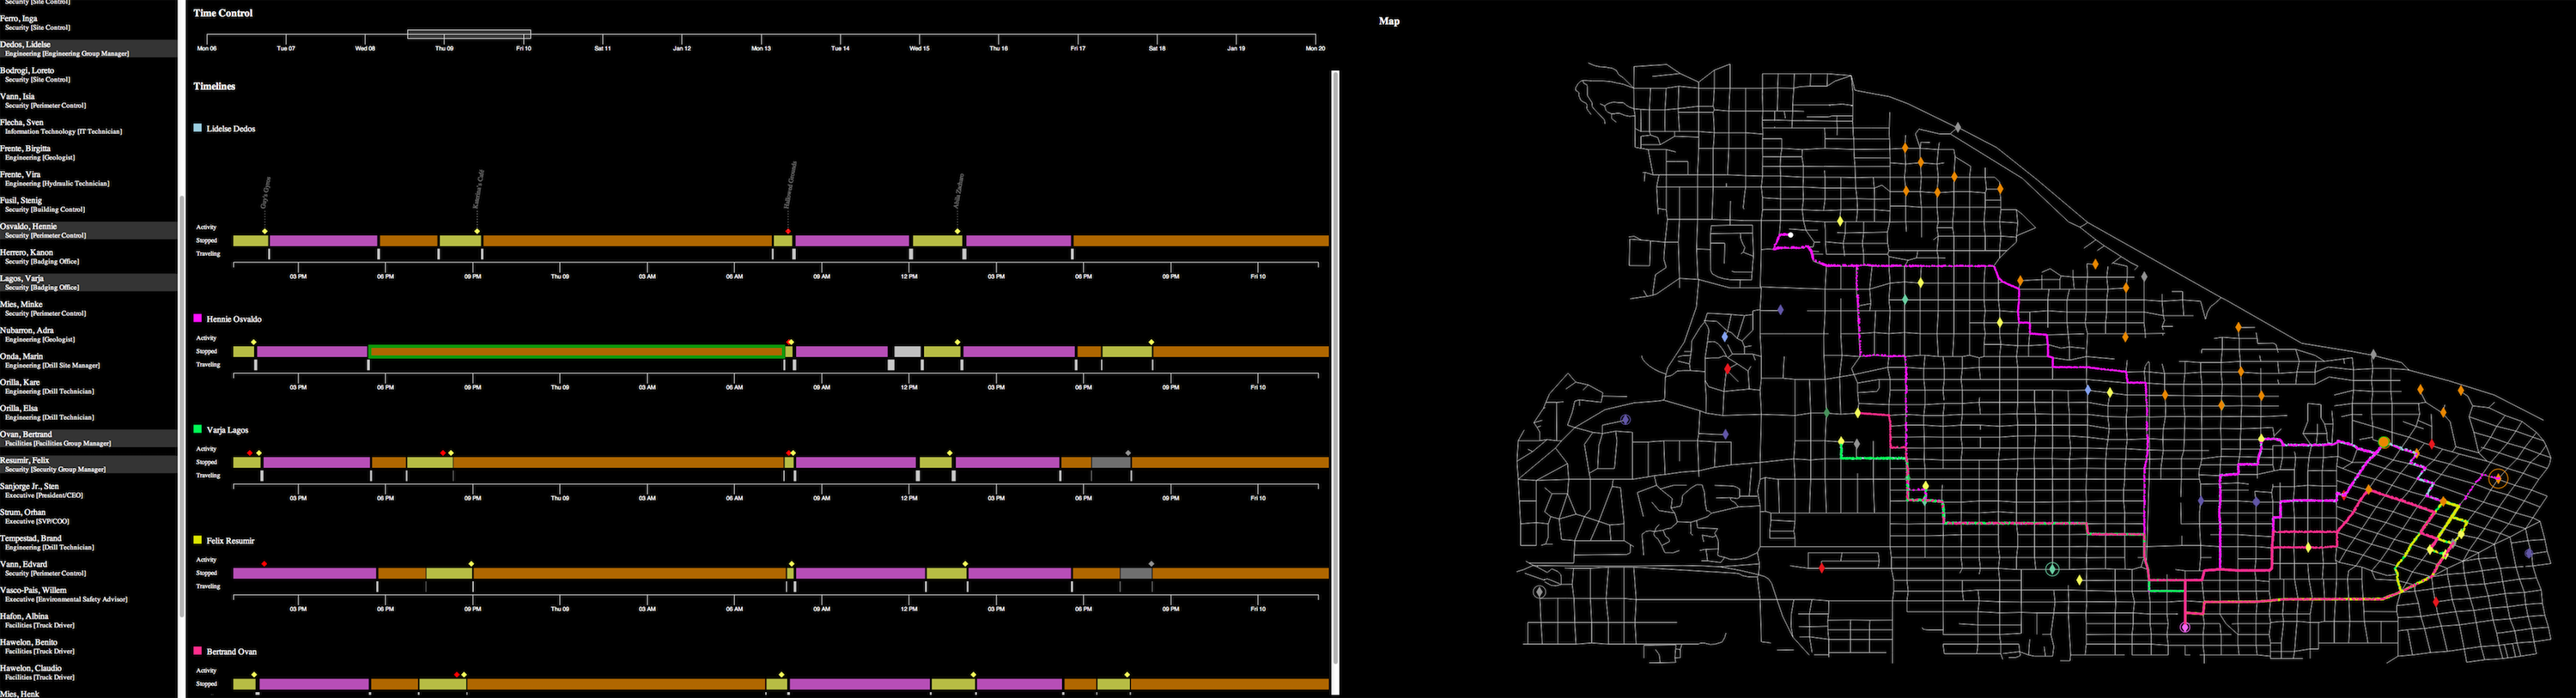
\includegraphics[width=1\textwidth]{vast-mc2-2014-cropped-scaled}
  \caption{The web interface for Andrews and Silver's VAST 2014 entry. The
  visualizations, from left to right, are a list of people, a master brushable
  timeline and individual timelines for each person listed with selectable
  events, and a map of GPS traces from the individuals' cars.}
  \label{fig:vast2014}
\end{figure}

For an example of the flow and feedback loop between preprocessing scripts,
back-end server, and front-end visualizations we look how we used the
Mini-Challenge 2 geographical data to identify points of interest and associate
them with car destinations. The VAST 2014 Mini-Challenge 2 dataset included
vehicle tracking data from company cars, an ESRI shapefile of the island where
GAStech is located, and an illustrated tourist map of the island. Tracking data
contained lists of latitude, longitude, timestamp, and car ID.

We wrote a preprocessing script in Python to iterate through individual
cars' GPS traces from the vehicle tracking data, identify periods where a car
was stopped, and save the coordinate where the car stopped as a destination for
the associated car. On the front-end, an interactive visualization rendered the
shapefile and preprocessed tracking data to draw a map of the city overlayed
with cars' movements and destinations. We created points of interest on the map
using car destinations and names from the tourist map. Persisting the
association of point of interest and a single destination to the database ran a
procedure that identified other nearby destinations to automatically associate
with the same point of interest.

Our VAST 2014 submission was unsuccessful. Working on the tool took most of the
available time and we were not left with sufficient time to complete the
investigation and write up the results.

\subsection{MiddGuard: Summer 2014}

The first version of MiddGuard, which was developed in response to summer
research at Middlebury, attempted to generalize parts of the web server and
front-end that could be reused throughout multiple investigations, while keeping
the framework unopinionated with respect to the data it could handle.

From the VAST 2014 Challenge we drew conclusions that influenced the first
version of MiddGuard. We found that the while the web could be an effective
platform for visual analytics, the overhead of creating custom tools, getting
those tools to work with the rest of the system, and implementation bugs in the
server-client communication hindered our progress investigating. To address
these issues, the framework's primary features were automatic persistence to a
database, data transport between the server and connected web clients in
real-time, centralized data storage in the web browser, and visualization module
loading/unloading in the browser.

This version of MiddGuard achieved flexibility by automatically loading three
types of customizable packages. These were referred to as analytics, modules,
and models. Analytics were scripts that could be triggered by a remote procedure
call from a front-end visualization. They could be passed data from the
front-end. Using the VAST 2014 example, they were meant to handle computations
like finding other destinations near a point of interest.

Modules were front-end visualizations that used JavaScript and CSS to render and
style elements in the browser's DOM. Visualizations were interactive, could
communicate with the backend to update and persist data, and could save state to
a global state handler to link visualizations to each other. For example, a
master brushable timeline saves the boundaries of the brushed region to its
state, which other timelines read to update their detail view.

Models were table-level schema for the database, intended to allow MiddGuard to
work with any data. A database table could then be created from each model. The
entire database was accessible on the front-end, with each table represented by
a Backbone.js Collection, which acts like an array of table rows. Collections
were updated in real-time using a publish-subscribe like method. Updates to a
collection on the front-end and to a models on the back-end were communicated to
one another in real-time. This allowed investigators to modify the data in
visualization modules and analytics packages without implementing communication.
By listening to changes in a Collection, a visualization could rerender as soon
as data changed on the server or in another investigator's browser. The
real-time, database-persisted communication protocol for models allowed
investigators to collaborate synchronously and asynchronously.

\subsection{VAST 2015}

Christopher Andrews and Jullian Billings used MiddGuard for the VAST 2015
Challenge. They report that the framework allowed them to take a modular
approach to developing tools for the investigation, deploying visualizations as
needed without needing plan and coordinate the entire investigation before it
began. They expanded the front-end state manager and used it to link their
visualizations: ``The shared state provided by Middguard meant that the modules
could be easily snapped together into an integrated environment, facilitating
the flow of information between the tools. This sped development because tools
could be simple and focused, with data selection and filtering shared between
tools.'' \cite{middguard-dinofunworld}. MiddGuard was well received by visual
analytics professionals, winning a VAST 2015 Challenge award for integrated
analysis environment.

The VAST 2015 Challenge investigation revealed some shortcomings of MiddGuard.
Storing all data in a web browser wasn't realistic. Datasets for investigations,
including VAST, are often several gigabytes in size, more than can fit in the
browser while maintaining the performance required for interactive
visualizations. Even with modifications to load subsets of the data, the
Backbone Collections quickly grew large, and filled with unnecessary data not
reflected in any active visualizations. View Reference Counting was designed to
address this issue.

Analytics packages, one of MiddGuard's built in tools for extensibility,
designed to run arbitrary code via remote procedure calls from the front-end,
were not sufficient to obviate the need for preprocessing scripts. The
investigators still wrote Python scripts to transform data and alter the
database outside MiddGuard. The lack of record of how these scripts were used
added a layer of opaqueness to the analytic process, making results hard to
reproduce and collaboration difficult. The framework designed and implemented in
this thesis addresses the issues of transparency and reproducibility in the
analytic process, while introducing a method to include the preprocessing script
contents in MiddGuard.

\subsection{View Reference Counting}

In the original implementation, one of the MiddGuard's weaknesses was handling
large amounts of data on the front-end. The framework was implemented to load
the entire database into the browser with the idea that investigators would need
access to all data during the investigation. MiddGuard's server would continue
to push data updates to connected clients as they became available. However,
with the large dataset from the VAST 2015 Challenge, the browser was not able to
handle all the data at once. MiddGuard was modified with a stopgap solution
during VAST 2015. Instead of loading all data from the outset, visualization
modules made custom database queries as necessary.

This did not solve the problem of unused data in the browser. Once downloaded to
the browser data was never removed, even after the visualization that required
it was. MiddGuard stores all data in a central location to avoid the duplication
that would occur by having each visualization store its own data. This makes it
impossible for a visualization that has requested data to clean up after itself.
Another visualization may have requested and currently be using the same data.

To keep the deduplication advantages of central storage and clean up after
visualizations that were removed from the browser, we implemented automatic
memory management in the browser called View Reference Counting. View Reference
Counting (VRC) maintains an array of references to the views that use each piece
of data as an attribute on the datum's Backbone.js Model. When a visualization
(a Backbone.js View, hence the name) is removed, its reference is removed from
the model. When a model has no view references it is removed from the browser.

Figures \ref{fig:vrc} and \ref{fig:vrccropped} demonstrate the efficacy of View
Reference Counting through the three memory snapshots taken by the Google Chrome
DevTools Memory Profiler. After a view with several megabytes of data was added
and removed, MiddGuard cleaned up the data and the browser was able to reclaim
the memory.

\begin{figure}[!ht]
  \centering
  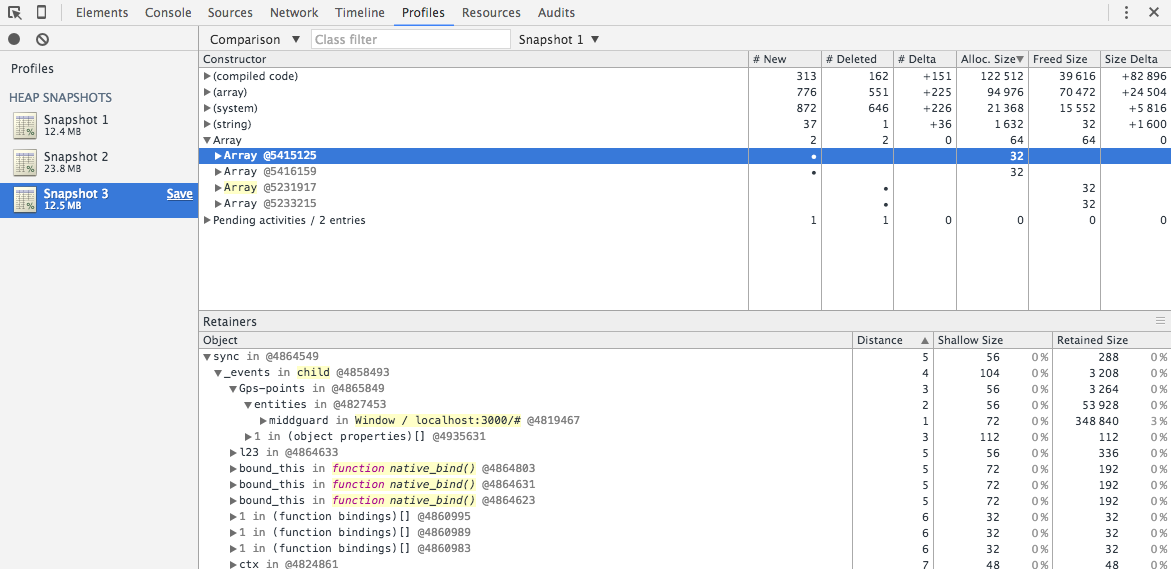
\includegraphics[width=1\textwidth]{devtools-snapshot}
  \caption{A screen capture of the Google Chrome DevTools Profiler demonstrating
  the efficacy of View Reference Counting. The panel on the left shows three
  snapshots. Snapshot 1 was taken before a view has was added. Snapshot 2 was
  taken after a view was added and rendered with a significant amount of data
  loaded into the browser. Snapshot 3 was taken after that view was removed and
  the memory was reclaimed.}
  \label{fig:vrc}
\end{figure}

\begin{figure}[!ht]
  \centering
  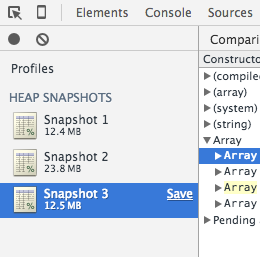
\includegraphics{devtools-snapshot-cropped}
  \caption{The snapshots portion of figure \ref{fig:vrc}, cropped for
  readability.}
  \label{fig:vrccropped}
\end{figure}

\chapter{Background}

\section{State of the Art}

Jigsaw \cite{Stasko:2008:JSI:1466620.1466622} is a visual analytics tool to
explore and understand collections of text documents. Introduced in 2007, Jigsaw
provides four visualizations, called views, to present different perspectives of
the text and extracted entities. While MiddGuard is not a text based tool, the
concepts that drive Jigsaw's views are of interest. Jigsaw views are coordinated
and communicate with each other to update themselves. User interaction with one
view updates the others. Multiple copies of each view can be created to reflect
different perspectives of the data.

MiddGuard supports customizable views, rather a limited, baked in, set. Like
Jigsaw, MiddGuard allows multiple copies of each type of view to be added to the
investigation, each with a different view of the data. MiddGuard visualizations
can be coordinated using a global state manager. Like the views themselves,
coordinations need to be developed manually.

Improvise \cite{weaver-2004a} enables users to build and browse
highly-coordinated visualizations interactively. It allows users to load data,
create views, specify visual abstractions, and establish coordinations
interactively. MiddGuard implements a similar build and browse system, where
visualizations are assembled using a visual configuration and simultaneously
rendered in the browser. Improvise places strong emphasis on complex,
scriptable, and visually representable coordinations between views where
MiddGuard relies on a global state manager, which developers can use as
necessary to coordinate multiple views.

Eagle Eyes \cite{7347662} is an interactive dataflow engine. Customizable
modules that can be chained together to transform, query the data, and create
visualizations. MiddGuard's data-flow model follows a similar data-flow model,
extending it through a synchronous collaboration system that allows multiple
analysts to work on the same data-flow at once.

\chapter{The Framework}

\section{Overview}

MiddGuard is a web framework that enables software developers and analysts to
create the tools to conduct complex, data-driven investigations. It provides a
browser based front-end and web server back-end on top of which developers can
build customizable tools specific to their data and investigation. Data is not
uniform and investigating that data requires bespoke tools. MiddGuard,
rather than implementing all the specific tools necessary to address all
possible scenarios, provides the scaffolding on which developers can bring and
build their own tools. The user interface and web server that MiddGuard
implement create a simple environment to connect and use those tools
transparently and efficiently.

MiddGuard breaks the operations of a visual analytics based investigation into
two general steps: data transformation and data visualization. Data
transformation involves any function on the data that results in a different,
possible destructive, representation of the same dataset. These functions might
involve reading, filtering, aggregating, annotating, or reformatting the
dataset. As a general rule in MiddGuard, if the operation does not produce a
visualization, it is a transformation. Data visualization takes place after the
transformation steps, creating a visual, often interactive, representation of
the dataset. By implementing these two steps, developers can extend MiddGuard to
fit their data and investigation.

These extensions to MiddGuard are called modules. Modules are short pieces of
code that often live in a single file. We divide modules into two types to
represent data transformation and visualization respectively. The former is
called an analytic module, while the latter is a visualization module. Modules
implement a simple protocol that MiddGuard is able to read and use to integrate
the code into the framework. Analytic modules consist of code that runs solely
on the web server. Visualization modules contain code that runs in the web
browser to render DOM elements that make up its visualization.

Once the MiddGuard web server is running, investigators use these modules to
build a data-flow graph. Modules are the graph's nodes. Edges between nodes
describe data-flow from module to module. MiddGuard's web front-end comes with a
graph editor that investigators use to add modules to the graph and connect
modules to each other. Once added to the graph, a module has been instantiated
in the context of the graph and is called a node. Analytic nodes can be chained
from one to the next, making the graph a canvas to compose complex data
transformations from multiple analytic modules, each with a singular task.
Visualization modules can be connected to analytic nodes, which feed in data to
create the visualization.

Although modules are customizable and can be written for a particular
investigation, they are also reusable within the same graph, different graphs of
the same investigation, or multiple different investigations. Modules'
relationships to each other are managed by MiddGuard and defined by connections
in the graph, rather than hardcoded into the modules themselves. For example, a
developer could create a visualization module that renders a heatmap of two
entities' activity moving around a city. The module would be written to accept
input from Entity A, Entity B, and the data to draw the underlying city map. An
investigator can connect the heatmap to any two cars, people, bikes, etc. from
another dataset and render a heatmap with no additional development effort. As
developers and investigators use MiddGuard, they build up a library of these
reusable tools. In a an investigation where time is a factor, being able to
quickly plug in and test data transformations and visualizations promotes the
investigator's efficiency.

\section{Example: Using Tweets to Investigate Relationships}

An example of the data-flow model is using tweets to determine the relationships
between multiple people: Alice, Bob, and Carlos. We start by writing three
similar modules that use a JavaScript library to access the Twitter API and
download all of the tweets for each person, respectively. Between the three
modules we only need to change the Twitter handle for which we are downloading
tweets. We add a graph called ``Tweet Relationships'' then create nodes from
these modules and add them to the graph. We can use the number of times one user
mentions (such as @Bob) another as a metric for the relationship, so we write
another module called ``Mention Count'' that extracts mentions from each tweet
and creates a mapping from the Twitter user mentioned to the number of times
mentioned throughout the dataset. We add this module to the graph three times,
and connect one ``Mention Count'' node to each of Alice, Bob, and Carlos's tweet
download nodes. Already we are able to reuse ``Mention Count'' for each person's
tweets. Finally, we visualize the relationships. We can use a force directed
graph with a node for each person and strength of the edges proportional to the
number of times one mentioned the other. Our visualization module, ``Force
Directed Graph'' will take three inputs, one for each person. We create a node
in the graph from the ``Force Directed Graph'' module and connect each of the
outputs from our ``Mention Count'' nodes to the three inputs of ``Force Directed
Graph''. Like the ``Mention Count'' module, ``Force Directed Graph'' is reusable
and can be plugged into any three inputs.

At this point our graph is ready to produce data and a visualization. We work
from the data entry points to the visualization, running the tweet download
nodes, then the ``Mention Count'' nodes, then the ``Force Directed Graph''
visualization. The analytic nodes report when they are done so we know it is
safe to run their dependents. Running the node ``Force Directed Graph'' renders
the visualization next to our graph in the browser window.

\section{Collaboration}

MiddGuard not only enables single investigators to create and work with these
tools, but also has built in support for asynchronous and synchronous
collaboration between teams of investigators. The framework includes user
registration and authentication so multiple investigators can create accounts,
log in, and work on the same investigations with the same graphs and access to
the same data. All configuration and transformed data is persisted to a
database, so investigators can log in and work with each other asynchronously,
one picking up where the other left off. Investigators can also work together in
real-time. As edits to the data-flow model are persisted to the database, they
are pushed to all connected web clients and the user interface updates without a
refresh to reflect those changes.

Since developers can collaborate to build the investigation, it follows that
they should be able to collaborate to record conclusions from their analysis.
MiddGuard comes with an observations tool for investigators to record and share
observations about the analysis, creating a chronological record of what
investigators saw in the data and when they saw it. An investigator of the
tweet-based relationships from the previous example might record ``Alice appears
to have a close relationship with Bob. See the Force Directed Graph
visualization in the Tweet Relationships graph.'' Like graphs and data, these
observations are persisted to the database and pushed to all connected clients
in real-time.

\chapter{Implementation}

\section{Technology}

MiddGuard builds on many open source software projects, some of which are
instrumental to its implementation. Node.js, Knex.js, and Backbone.js make
possible MiddGuard's structure and flexibility.

Node.js \cite{nodejs} is an asynchronous, event-driven JavaScript runtime built
on Google Chrome's V8 JavaScript engine. The runtime is structured around an
event loop where callbacks are registered and fired later in the program's life.
Most I/O operations are performed indirectly through the event loop, so the
process rarely blocks, allowing high concurrency and scalability. MiddGuard's
server is implemented in JavaScript running on Node.js. The code for its HTTP
and WebSockets, servers take advantage of the event loop. WebSockets are a
bidirectional protocol for client-server communication. Since they are
event-driven from the server, rather driven by the HTTP request-response cycle,
WebSockets are simpler to implement and deploy with Node.js than with many
traditional servers for other languages and web frameworks.

Knex.js \cite{knexjs} is a SQL query builder with support for several relational
databases including Postgres, MySQL, and SQLite. Knex exposes an API with
function calls similar to SQL keywords that generate and execute SQL in the
appropriate dialect for the connected database. It supports schema generation
and returns the results of queries it runs on the database. MiddGuard uses
Knex.js to simplify database connections for custom analytic modules and make
the framework flexible to whichever database is best suited to the
investigation. For the VAST 2015 Challenge Andrews and Billings used a Postgres
database and connected over the network to collaborate from separate machines
using the same database. For single person investigations using SQLite is often
preferable since it does not require a database connection.

Backbone.js \cite{backbone} is a front-end library designed to give structure to
web applications. It consists of extendable Models, Views, and Collections, all
of which we use to structure MiddGuard's front-end. Models manage data
attributes and trigger events when that data changes. Collections are groups of
related models. For example, there may be a Model called \textit{Book} with
attributes \textit{title} and \textit{author} and a Collection called
\textit{Library} that contains multiple books. Collections also emit events when
updated. Both Models and Collections can persist their state to a web server
that implements a REST API over HTTP. MiddGuard replaces the REST API
persistence with a similar one implemented with WebSockets. Backbone.js Views
are pieces of user interface. They render HTML in the browser and listen to
events emitted from Models and Collections to update themselves. MiddGuard's
front-end user interface is implemented using Backbone.js Views. Visualization
modules extend a MiddGuard View, which is inherited from a Backbone.js View, to
support View Reference Counting and automatic layout in MiddGuard's browser
environment.

The browser, front-end, client, and other variants are all used to refer to the
web browser, where MiddGuard's user interface lives. The browser is a
non-traditional environment for visual analytics, which are often implemented as
desktop applications to achieve higher performance through OS native code over
JavaScript which runs non-natively in the browser. However we were inspired by
the expressiveness and ease with which we could create interactive
visualizations with tools like D3.js \cite{2011-d3}, a JavaScript library for
manipulating HTML, CSS, and SVG in the DOM based on data, and decided to
implement MiddGuard as a web application.

\section{Data-flow Model}

MiddGuard's data-flow model allows arbitrary nodes, each with their own idea of
input and output, to be chained together in a graph of data transformations and
visualizations. Nodes are reusable units of code, so multiple instances of the
same type of node, or module, can coexist in a single investigation. Connections
between nodes allow data to pass between them.

\subsection{Analytic Nodes}

One of the issues with the first version of MiddGuard was no integrated way to
create and represent the preprocessing scripts used to transform data before
visualization. These scripts did most of the work to setup and populate the
database, so they were a major component missing from MiddGuard's idea of the
analytic process. Nodes address this problem, creating a flexible representation
within MiddGuard of the data processing phase of an investigation. In this
section we will address the implementation of analytic nodes. Visualization
nodes and their differences with respect to analytic nodes will be addressed in
a subsequent section.

Analytic nodes are instances of modules, made unique from one another by the
data they generate. MiddGuard is backed by a relational database where nodes are
each assigned their own table. They use this table to persist their data. Nodes
generate their data using their module's handler function, invoked from a button
press in the user interface. Nodes can be created throughout an investigation
and multiple nodes can be created from each module, so a node's table is created
just before its handler is called.

Analytic modules specify a function that will be used to create all of its nodes
tables. That function is passed in the name of the table to create and a
connection the the database in the form of an SQL generator called Knex.js
\cite{knexjs}. The function uses the connection and table name to generate the
schema for its tables.

Nodes are not standalone scripts, they can work together to perform complex
transformations, just as a developer might run one script after the other. Each
node can output its data and receive input from other nodes. Inputs and outputs
are passed into the node's handler function so it can use one to generate the
other. The combination of input and output is a node's \textit{context}.
Creating a node's contextual output involves only the node itself. Every node
has exactly one output, its own table. Other nodes that receive input from it
are simply querying that table. The output passed into a node's handler is a
Knex.js database connection already assigned specifically to perform statements
on the node's table. Creating a node's contextual inputs, however, requires
analyzing its connections to other nodes.

\subsection{Connections}

Connections a two-level protocol of node to node connections and
intra-connection name mappings, used to determine the input passed into one node
from another. Each node can have multiple named inputs, referred to as
\textit{input groups}. Each input group can have exactly one connection to
another node, referred to as an \textit{output node}. We refer to the parent
node of an input group as the \textit{input node}.

A mapping from an input group to an output node creates a mapping from that
input group's name to the output node's table. This mapping is stored as a
key-value pair where the key is the input group, and the value is the output
table name.

When MiddGuard generates the contextual inputs for a node, they key value
mapping allows developers to use the input group names they picked for the
module to look up the values to access the input data. For the input context,
the table name is translated to a combination of table name and a Knex.js
accessor. The table name, while unnecessary for queries that only use that
table, allow full flexibility for more advanced queries, such as table joins.

Input group to output node mappings tell us where a specific input's data lives,
but not what the data looks like or how to refer to it. That is, we have the
table to look in, but we don't know what its schema is and in particular, what
its columns are named. Unless the only SQL we want to run is \texttt{SELECT *
FROM `output table'}, we need more information.

We address this at the second level of our connection protocol: intra-connection
mappings within the input group to output node connection, that identify the
column names in the output table. This is another set of key-value pairs that
map the names the input node has assigned to each attribute in an input group,
to the corresponding column to access in a the output table. When generating the
contextual input for a node, this mapping is included for each input group. Like
at the higher level of input group mappings, developers can look up the the
output table column name using a key they pick to represent that attribute.

Listing \ref{lst:connectionjson} shows an example connection configuration for a
node called ``Time by Day/Hour'' that aggregates data by day of the week and
hour of the day. The configuration for ``Time by Day/Hour'' has one input group,
called ``tweets'', which is connected to the output node with id \texttt{9}. The
\texttt{output\_node} field serves as a foreign key referencing another row in
the same table. The column-level connections between the input group and output
node \texttt{9} are stored within the input group. Column mappings are stored in
an array called \texttt{connections}. Each object within the
\texttt{connections} array has an a key \texttt{input} and a key
\texttt{output}. The value of \texttt{input} is the name the input node has
given to the column and the value of \texttt{output} is the name the output node
has given to the column.

\begin{lstlisting}[caption={A node's connection configuration. The node has a connection from its input group ``tweets'' to the node with id 9.}, captionpos=b, label={lst:connectionjson}]
{
  "tweets": {
    "output_node": 9,
    "connections": [
      {
        "output": "handle",
        "input": "handle"
      },
      {
        "output": "tweet",
        "input": "tweet"
      },
      {
        "output": "timestamp",
        "input": "timestamp"
      }
    ]
  }
}
\end{lstlisting}

\subsection{Connection Storage}

The connections generated within the graph editor are stored in MiddGuard's
table of nodes, as a JSON string in the same row as their corresponding input
node. We considered multiple factors when deciding how to store connections in
the database. We wanted a storage method that was portable, efficient, and
convenient. Portability meant that we could easily export the configuration of
nodes and connections to a text file so they could be read back in and the graph
could be reassembled in a different system. Efficiency was determined by the
number of database operations required to access the configuration. This was
important since we have to read and write connections whenever a node is
accessed or modified in the graph editor. Convenience meant that it was not
overly complex to access and modify the connections from a programming
perspective.

In addition to the JSON string storage method we implemented, we considered
storing connections and nodes in separate tables, with either each column-level
connection in its own row or each group of column-level connections in a row.
The former performed no grouping amongst column mappings, while the latter
grouped each input group's columns in a single row.

The first option (each column mapping has its own row) was appealing since it
took advantange of the relational database, using foreign keys to associate
column mappings with their nodes. However, this method is less portable since it
requires multiple steps to export all the node information and their associate
column mappings from the database to a structured text file. It is also less
efficient since it requires reading a row from the database for every column
mapping, in addition to a row for every node. Finally, it would be less
convenient to develop with because it would require more queries to the database
to obtain all the information to construct the graph than if we stored the
connection information close to the nodes.

For similar reasons, we ruled out the second option of storing all column level
connections in a row, grouped by their input group. This seemed like a poor
compromise between storing all column mappings separately and storing all
connection information with their nodes. We would lose the elegance of
conforming to the facilities of a relational database, and still have to query
the database multiple times to assemble a graph or export/import the data.

The implemented method of storing a node's connection in the same database table
row as the node, in a JSON string, satisfied all our requirements. It is
portable: JSON is common format to export human readable configuration. We can
simply query all nodes and write out their metadata and JSON string as
connections. It is efficient to access nodes and connections to construct a
graph. All of a graph's nodes and connections can be accessed by reading
\textit{n} rows from the database, where \textit{n} is the number of nodes in a
graph. It is convenient to work with this format, since all the connection data
for a node can be obtained by calling JavaScript's built-in \texttt{JSON.parse}
method on a node's connections column.

\subsection{Context Generation}

A node's connections can be edited in the graph editor until runtime, when a
node's handler function is executed. At this point, MiddGuard makes a query for
the node in the database and retrieves its stored connections. Parsing the
connections JSON string lets MiddGuard access the mapping of input groups to
output nodes and the mappings of column names between nodes. MiddGuard makes
additional queries to determine the table names of connected output nodes. With
just this information, MiddGuard can construct the dynamically generated context
to pass into the handler function. Listing \ref{lst:nodecontext} is a sample of
the context passed into one of the same ``Time by Day/Hour'' nodes whose
connection was previously listed. At the top level it includes \texttt{inputs}
and \texttt{table}. \texttt{inputs} is an object mapping each of the nodes input
groups to data about the connected output node. Within \texttt{inputs} are:
\texttt{knex}, an instance of the Knex.js SQL generator \cite{knexjs}, used to
access the table connected to an input group; \texttt{cols}, the column-level
mapping between the node's input group and the connected output node's column
names; and \texttt{tableName}, the name of the connected output node's table
name. \texttt{cols} and \texttt{tableName} are meant to give access to the
information available for more advanced queries, such as table joins.

The other top-level key in the context, \texttt{table}, gives access to the
output table for this node. Like each input group in \texttt{inputs}, it has a
\texttt{knex} accessor to generate SQL to query the database, and a
\texttt{name}, which is the node's own table name. \texttt{table}, the output,
doesn't need a column mapping, since the column names are the same as the ones
the node has assigned itself as outputs.

\begin{lstlisting}[caption={The context passed into a ``Time by Day/Hour'' node's handler function.}, captionpos=b, label={lst:nodecontext}]
{
  inputs: {
    tweets: {
      knex: [Object],            // database connection instance
      cols: {
        handle: 'handle',
        tweet: 'tweet',
        timestamp: 'timestamp'
      },
      tableName: 'download-tweets-danarsilver_1'
    },
    table: {
      knex: [Object],            // database connection instance
      name: 'aggregate-time_2'
    }
  }
}
\end{lstlisting}

Having to make additional queries to access output nodes' table names is a
potential source of ineffiency not addressed by our connections storage format.
A way around this would be to duplicate the table name each time it appears in a
connections JSON string. We decided against duplicating the data and in favor of
making additional database queries instead to avoid fragmenting the information,
should the table name change. Should we need to update a node's table name, it
can be done once for the row, rather than having to update the connections
string in all other connected nodes.

\section{Visualization Nodes}

Our model for visual analytics is incomplete without the visualizations
themselves. We include visualizations in the data-flow model as their own nodes,
which we refer to as \textit{visualization nodes}. By integrating visualizations
into the data-flow model, we can pass data transformed by the analytic nodes
directly into our visualizations.

Visualization nodes, like analytic nodes, are added from modules in the graph
editor. They have input groups that can be connected to output nodes, and column
mappings between the two nodes on the ends of the connections. The primary
difference between analytic nodes and visualization nodes is that the handler
for a visualization node is a newly instantiated Backbone.js View
\cite{backbone} that is rendered in the web client.

The instantiated view for a visualization node has an instance method called\\
\texttt{createContext}, which can be called to dynamically generate the context
for a view, just as the MiddGuard generates the context for an analytic node on
the back-end and passes it into the handler function. The context for a
visualization node has the same structure as that of an analytic node, without
the output, since a visualization node's output is a visualization, rather than
a table of data.

Additionally, the Knex.js accessors for each input group are replaced with
instances of Backbone.js Collections (with a new key aptly named
\texttt{connection}), which can be used like the Knex.js accessor to access the
data from output node connected to that particular input. MiddGuard instantiates
a Backbone collection for each analytic node and a corresponding endpoint on the
back-end to transmit the analytic node's data to the collection, as required by
a visualization node.

Backbone.js and consequentially MiddGuard visualization nodes have are not
reliant on library or framework to manipulate the DOM and render a
visualization. This keeps MiddGuard flexible for any toolchain a developer wants
to use to create visualizations.

A potential improvement in the implementation of visualization nodes would be to
only instantiate collections for analytic nodes that output to visualization
nodes. Other nodes' data will never be accessed, so it is not necessary to
maintain collections on the front-end or the endpoints on the back-end to
transmit data to them. However, this is a low-priority improvement since there
is little overhead in terms of memory usage to create an empty connection on the
front-end or add the event listeners that handle data transmission to Node.js's
event loop on the back-end.

\section{Visual Programming}

Visual programming abstracts away the details of the data-flow model within
MiddGuard as descibed in the previous sections, and the independent
implementation details of each node. A major motivation for MiddGuard is to
facilite quick construction of complex visual analytic tools. MiddGuard's system
for visual programming allows investigators to quickly compose data
transformations and visualizations. The visual component creates an expressive
representation of the steps to reproduce a visualization.

The visual programming interface takes place in the three panels of the graph
editor, seen in figure \ref{fig:grapheditor}. The left panel, titled
``Modules'', lists all modules from which nodes can be instantiated. Clicking a
module's button in the list adds a node of that type to the canvas in the middle
panel.

\begin{figure}[!ht]
  \centering
  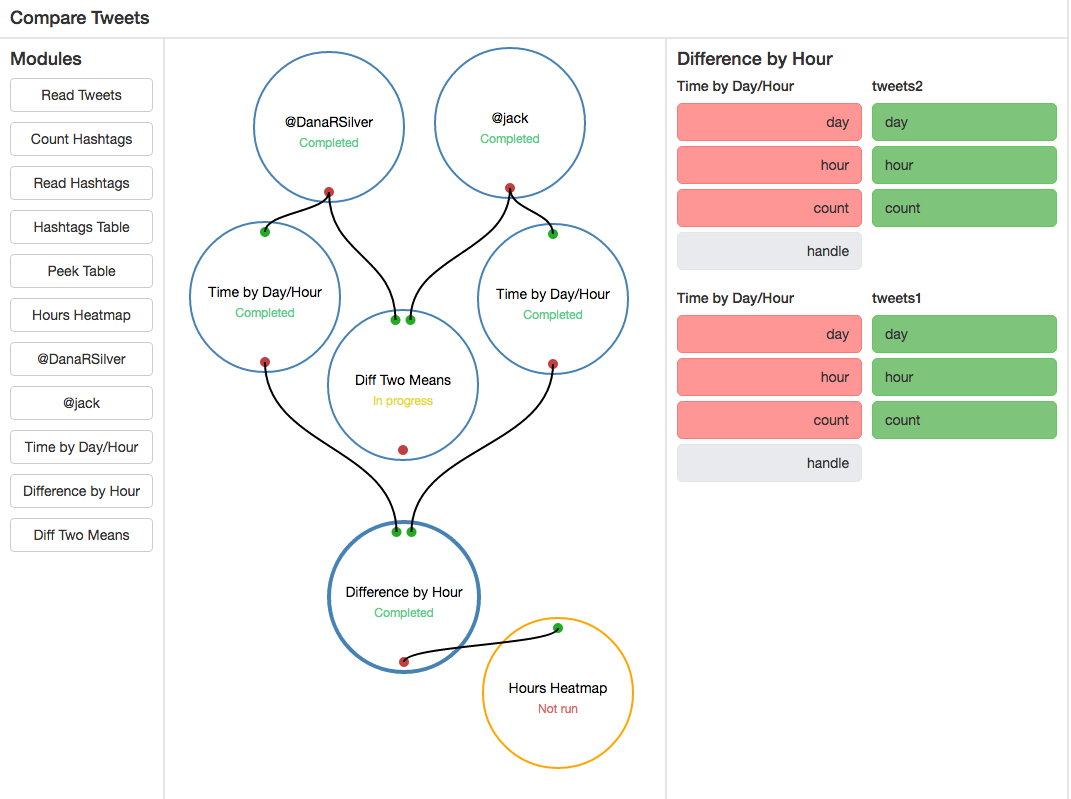
\includegraphics[width=1\textwidth]{compare-tweets-graph-editor-no-sidebar}
  \caption{MiddGuard's graph editor user interface, open on a graph named
  ``Compare Tweets''. On the left, the modules panel lists all loaded modules,
  from which nodes can be created. In the center, the graph editor canvas has
  seven nodes initialized from their respective modules, and connections between
  the nodes. On the right, the detail panel shows the column mappings between
  the ``Difference by Hour'' node and its connections to two
  ``Time by Day/Hour'' nodes.}
  \label{fig:grapheditor}
\end{figure}

The middle panel's canvas is a free-form space limited by the height of the
window and a 500 pixel width constraint. Nodes, once added to the canvas, are
outlined circles that can be rearranged and connected to one another. Analytic
nodes and visualization nodes are outlined in blue and orange respectively, to
make them easy to differentiate.

Figure \ref{fig:annotatednode} shows an analytic node with all its elements for
user interaction in view. The cross in the upper left corner is used to drag the
node around the canvas. Allowing nodes to be draggable is a simple solution to
problem of node layout. A downside is the additional effort and time required on
the part of the user to position and reposition nodes in the canvas, but this is
outweighed by both its simplicity to implement over a layout algorithm and the
flexibility for the user to customize the graph view as best appeals to their
idea of the investigation.

The ``play'' button, located in the top right of each node abstracts both
analytic and visualization nodes' action. In an analytic node clicking play
calls its handler function. In a visualization node, the play button creates a
new instance of a visualization. Pressing a visualization node's play button
again removes that visualization from the browser window. Like the graph
editors, stack horizontally in the browser window. The user can scroll through
them from left to right.

While web scrolling is typically done vertically, we implemented view layout
horizontally, since MiddGuard was designed to be used on the same system used
for the preliminary VAST 2014 and VAST 2015 investigations. These investigations
used a system of three 27 inch displays arranged side by side
\cite{middguard-dinofunworld}.

Each node contains two text indicators: in the center of the node in black is
the node's module type. This is a visual indicator of the operation that will
occur or visualization that will be rendered. Just below is the node's status
indicator, one of ``Not run'', ``In progress'', or ``Completed'' in red, yellow,
or green, respectively. The status indicates whether the handler function has
already been invoked. Investigators ultimately use the node's status to
determine when a visualization is able to be rendered in the browser. Only once
all a visualizations dependent nodes have been run and have a status of
``Completed'', can a visualization be rendered.

The connections between nodes' inputs and outputs are key components in the
visual programming interface. They represent connecting code paths and passing
data from one node to another. A connection can be created from one node to
another by selecting one green input group indicator seen at the top of the node
in figure \ref{fig:annotatednode} and one red output indicator like the one seen
at the bottom of the same node. The selected input and output connectors are
outlined with a black stroke. It is possible to connect a node's input to its
own output, however this would result in no operation since the data required
for the input would not exist at runtime. Since nodes can accept input from
multiple outputs, hovering an input group indicator opens a tooltip with the
name of the input group under the mouse to aid the investigator in creating the
correct mapping.

Clicking a node widens its outline and opens the node's connections in the
detail panel, seen on the right of figure \ref{fig:grapheditor}. The detail
panel lists each input group's column-level connections, grouped by that input
group, and organized so output columns are on the left in red, and input columns
are on the right in green. When a connection is made in the graph editor,
MiddGuard attempts to automatically match columns based on the names. Any
columns that don't match appear below the matched ones in gray. Columns can be
connected manually in the same way as nodes: by clicking to select an output and
an input to connect. The columns names in each group re-render to indicate the
pairing after the connection has been made manually.

The similarity between interactions to edit connections at both the node and
column level and the color coding of inputs and outputs in both the graph editor
canvas and the detail panel is intentional, meant to make graph construction
intuitive for an investigator. The goal of visual programming is to reduce the
complications for an investigator to create a complex program. A familiar, easy
to learn user interface promotes quick, simple development and reduces the
cognitive load devoted to MiddGuard as a tool rather than the investigation
itself.

\begin{figure}[!ht]
  \centering
  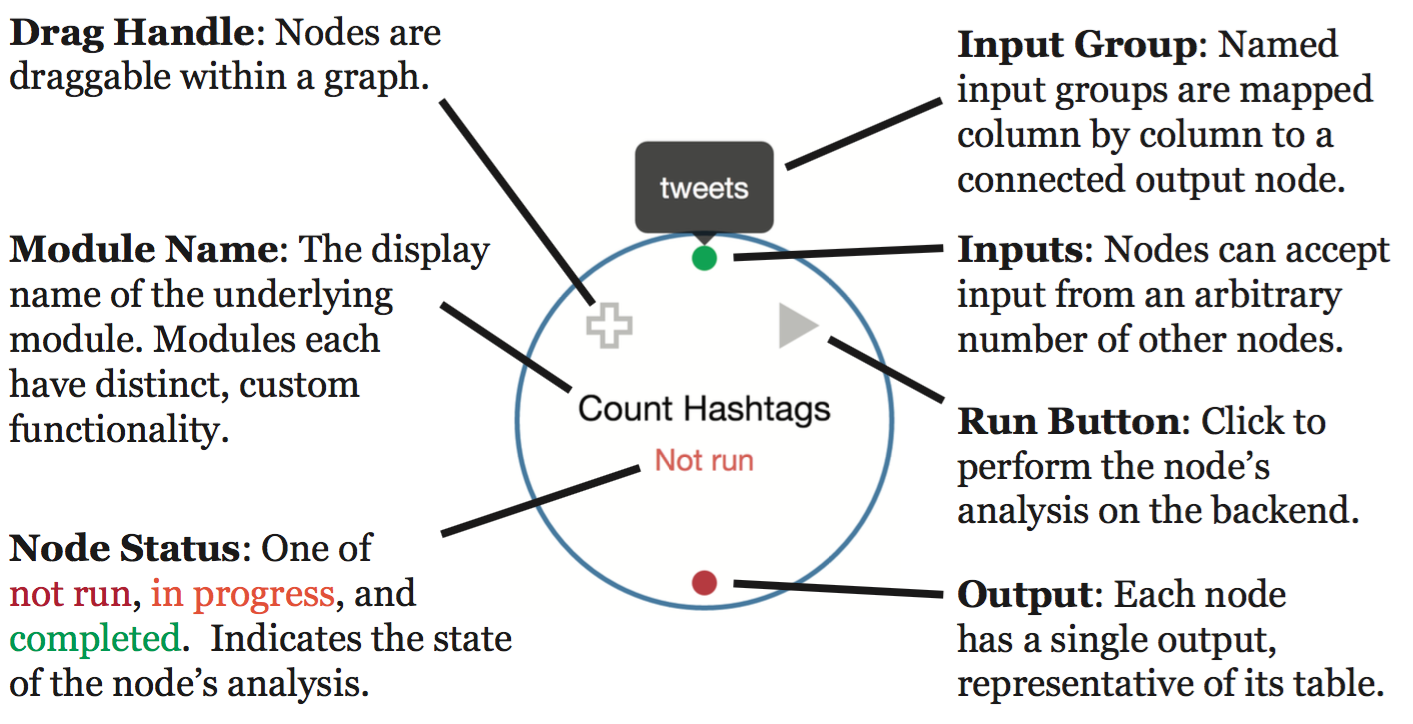
\includegraphics[width=1\textwidth]{middguard-analytic-node-annotated}
  \caption{An analytic node in a graph. Important features are annotated and the
  node's only input group, ``tweets'', is moused over to show its accompanying
  tooltip.}
  \label{fig:annotatednode}
\end{figure}

\section{Extensibility}

As mentioned before, the primary motivation for MiddGuard is to create a
framework that allows investigators and developers to quickly and effectively
create visual analytics tools. MiddGuard needs to be able to adapt to any
investigation with any types of data and visualizations. To support any data or
visualization, MiddGuard can register and load external code referred to as
modules. While visual programming is the user interface for analysts to quickly
put together an investigation with an expressive representation, the API for a
module is the user interface for developers who work with MiddGuard, and need to
quickly construct bespoke data transformations and visualizations.

Modules are the constructors from which nodes are initialized. They expose all
the metadata necessary to construct a node as well as the function or view that
will be called or rendered when the node's play button is pressed. Each node
contains a reference to the name of its constucting module so this metadata and
function can be accessed at runtime.

Modules themselves are short and designed to be written quickly. Figure
\ref{fig:analyticmodule} gives an example of an analytic module that bins tweets
by the day of the week and hour of their timestamp. This module performs the
final step of analysis in the ``Compare Tweets'' graph of figure
\ref{fig:grapheditor} before data is fed into the visualization.

An analytic module can be as simple as one JavaScript file that exports the few
objects as in figure \ref{fig:analyticmodule}. Those exports include an array
of inputs the module can accept, grouped by input group. Each input group
contains a list, \texttt{inputs}, of the attributes the module requires for each
member of the input group. The second export is an array of output attributes
for each member element the module will output.

The outputs correspond directly to the contents of the third export, a function
called \texttt{createTable}. The \texttt{createTable} function is used to create
the backing table for a node. All nodes

\begin{figure}[!ht]
  \centering
  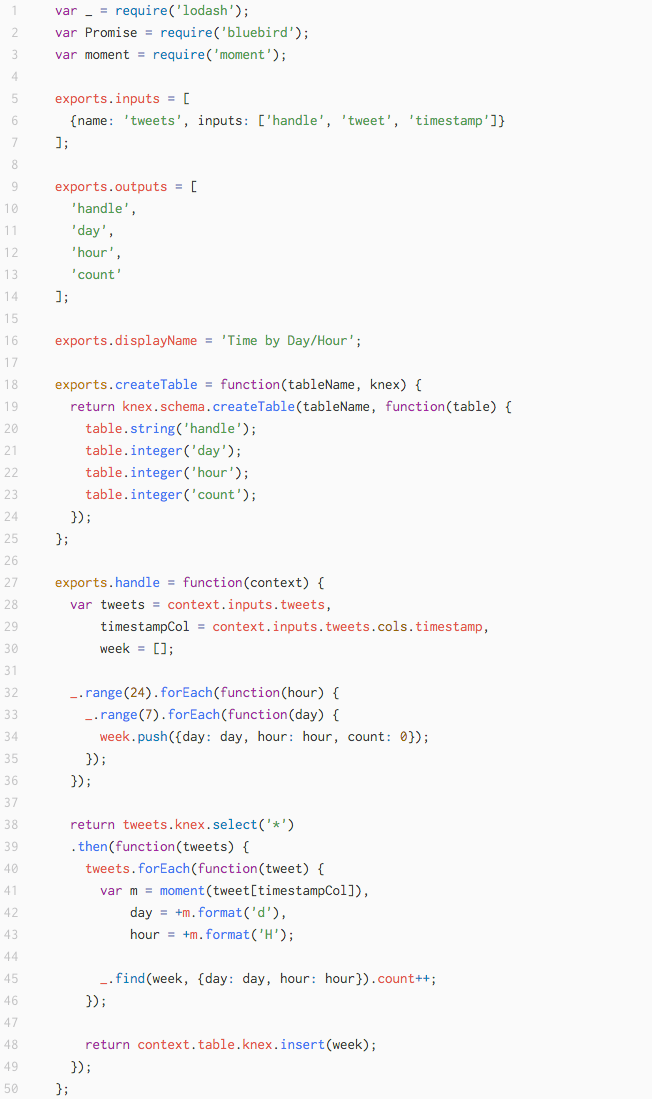
\includegraphics[width=.85\textwidth]{analyticmodule}
  \caption{Code for an example analytic module.}
  \label{fig:analyticmodule}
\end{figure}

\section{Real-time Collaboration}

MiddGuard supports asynchronous and synchronous collaboration between multiple
developers. Asynchronous collaboration is common in a web application. For
example, User A makes changes, which are persisted to a data store. User B logs
in some time later and the changes User A made are loaded from the database so
User B can view them.

Synchronous collaboration is more difficult to implement. Web application
communications are largely based on the HTTP protocol. Data is transferred from
the web server to the client in an HTTP session, which is made up of a request
from the client and a response from the server. The client must initiate an HTTP
request before the server can send data. This is problematic for real-time
communications. Like in the asynchronous example, User A might make a change,
which should be immediately pushed to all other connected clients. User A can
make an HTTP request to tell the server about the change, but there is no way
for the server to tell other clients about the change immediately. With HTTP,
User B must explicitly request the update, which requires either knowing when to
check for an update (unreasonable) or continuously polling the server for
changes (inefficient).

WebSockets help solve real-time communications, and are implemented in place of
HTTP for all of MiddGuard's server-client communications after a user is
authenticated and logged in. WebSockets is a bidirectional event-driven
communication protocol designed for browers and servers to exchange data without
relying on HTTP requests and responses \cite{mdn-websockets}. WebSockets are
layered on TCP. The connection from the browser to the server is initiated with
the HTTP Upgrade header and client-server handshake after the browser has
received a traditional HTTP response from the server with the code to perform
the Upgrade request \cite{RFC6455}.

The MiddGuard server registers WebSocket event handlers for its internal
components and for nodes' data. Data on the front-end is structured using
Backbone.js Models and Collections, which traditionally use HTTP to perform
create, read, update, and delete (CRUD) operations. We use third-party
libraries, Backbone.ioBind and Backbone.ioSync, to replace the HTTP requests
with a similar protocol using WebSocket events. A HTTP request \texttt{POST
/graphs} becomes \texttt{socket.emit('graphs:create', data)}. Emitted from the
the browser, these events offer no real advantage of their corresponding HTTP
requests. The use case for WebSockets is emitting events and data from the
server to the client, which is impossible over HTTP. With the connection open,
we can send events from the server to the client to create, update, and delete
(the server does not need to read data from the client) Backbone Models and
Collections whenever the data change on the server, enabling real-time updates
and collaboration for clients.

\chapter{Discussion}

\section{Use Case}

We constructed a small investigation into Twitter data to help implement and
test MiddGuard as we implemented the framework. Using tweets from two users'
timelines, we wanted to determine who tweets more each hour of each day of the
week.

To find an answer we wrote four analytic modules and two visualization modules.
Our first two analytic modules accessed the Twitter API to download tweets from
the two subjects, ``@DanaRSilver'' and ``@jack''. These are also the names of
the respective modules. Next, we wrote ``Time by Day/Hour'', which uses tweets'
timestamps to aggregate the them by day of the week and hour of day. Our last
analytic module, ``Difference by Hour'', computes the difference between counts
for each combination of day and hour and groups the two counts into a single
table. We created a new graph and and connected the ``@DanaRSilver'' and
``@jack'' nodes each to a ``Time by Day/Hour'' and fed those into a ``Difference
by Hour'' node. Figure \ref{fig:tweetanalysisgraph} shows the complete graph.

\begin{figure}[!ht]
  \centering
  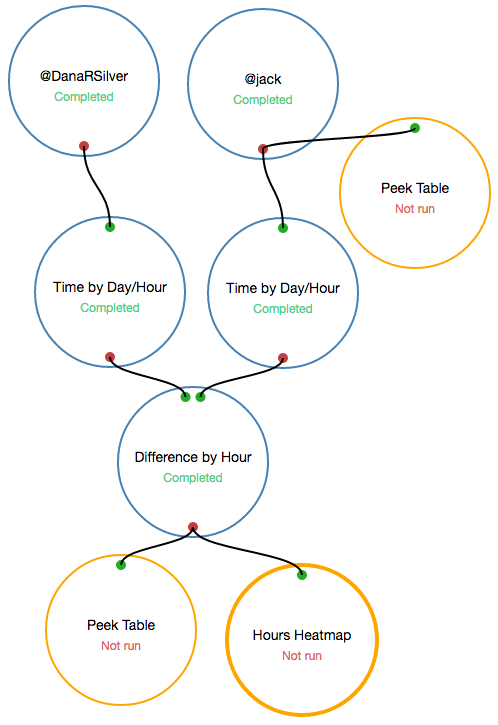
\includegraphics[width=0.75\textwidth]{tweetanalysisgraph}
  \caption{The complete graph from the mock investigation used to develop and
  test MiddGuard.}
  \label{fig:tweetanalysisgraph}
\end{figure}

Since our goal was to figure out who tweets more at each combination of hour of
the day and day of the week, we wrote a visualization called ``Hours Heatmap'',
a bubble chart with hours on the x axis and days on the y axis (Figure
\ref{fig:punchcard}). Two circles, or bubbles, are drawn at entry in the chart,
one for each person. The circles' radii are mapped to the number of times the
corresponding person tweeted that hour and day. Mousing over a pair of circles
adds a tooltip with the exact count.

\begin{figure}[!ht]
  \centering
  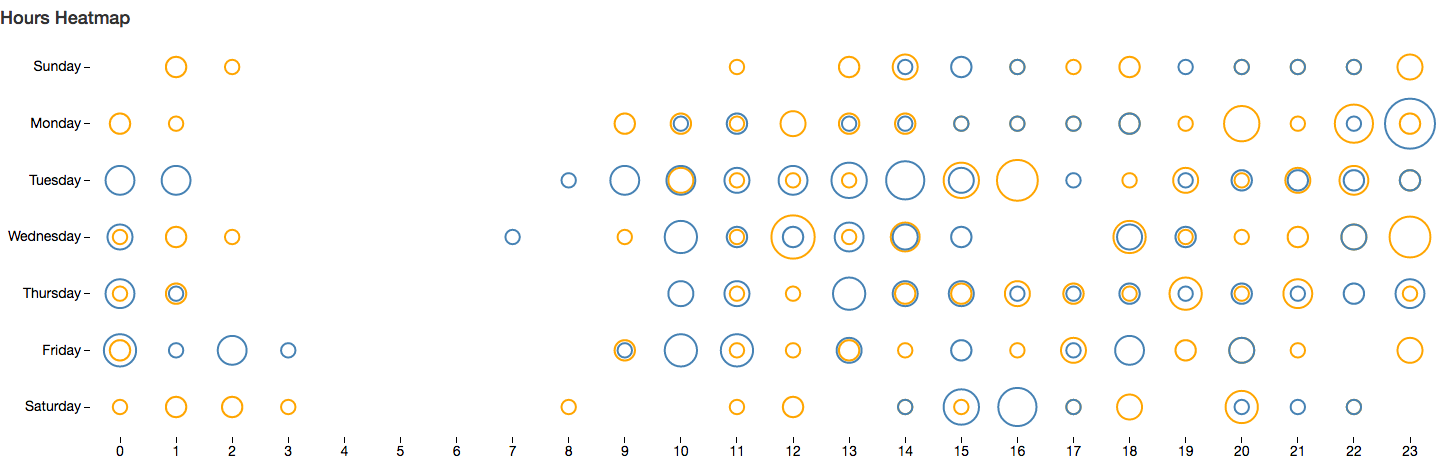
\includegraphics[width=1\textwidth]{punchcard}
  \caption{The ``Hours Heatmap'' visualization from the mock investigation used
  to develop and test MiddGuard. @DanaRSilver's tweets are orange, @jack's are
  blue. Circle radii are mapped to the number of times each person tweeted in
  that hour and day of the week.}
  \label{fig:punchcard}
\end{figure}

From the ``Hours Heatmap'' visualization we are able to answer our question. We
can look to any particular day and hour and see who tweets more. Wednesday at
12pm, for example, Dana tweets more than Jack. Dana tweeted nine times and Jack
tweeted twice. We are also able to identify some patterns in the tweets. Both
people rarely tweet late at night, and never between 4am and 6am. Jack is more
active on Saturday than Dana and both get a late start on the weekends.

While we were investigating our primary question, we wanted to look at the data
we received from the Twitter API as well, to make our investigation more
transparent, and to test that we had downloaded tweets correctly without having
to work with the database outside MiddGuard. We wrote a visualization ``Peek
Table'' that takes any input and renders it as a table. We hooked this up to
both the ``@DanaRSilver'' and ``@Jack'' modules and could immediately tell that
our download had worked as intended. Since we could see the text of the tweets,
we could also see that Jack retweets much more often than Dana.

\section{Areas for Improvement}

The mock investigation into @DanaRSilver and @jack's tweets revealed two areas
for improvement in MiddGuard. The first is that modules only can change context
from between nodes with respect to the incoming and outgoing data. We have two
almost identical modules to download @DanaRSilver's tweets and @jack's tweets.
The only difference is the Twitter handle accessed. When one of our goals is
reuse of the data transformation logic, it does not make sense to repeat logic
just to change a variable. We could improve on this by allowing developers to
define variables that can change from node to node and create an interface for
investigators to define that variable for the node. This would have allowed us
to write one module that downloads tweets, create two nodes from it, and pass
``@DanaRSilver'' and ``@jack'' in as variables.

Developing the modules was challenging, since it was hard to test if the
transformation logic worked. We eventually created the ``Peek Table''
visualization module to check the table contents, however this required creating
multiple nodes and running the user interface to test. There is no way to remove
data from a node, so if the transformation was applied and saved data
incorrectly, additional nodes would have to be created to test the module again.
This issue could be solved with a procedure to pass data through a module
without creating a node in the user interface, and without persisting that data
to the node's table. Besides simpler development, this solution would make it
substantially easier to write tests for modules, which in MiddGuard's current
state would require creating a database, starting the web server, and
manipulating the user interface in a web browser.

Outside the areas of improvement discovered during the use case, MiddGuard could
be improved to better incorporate visualization nodes into the data flow.
Visualization nodes should be able to modify data in the database and have their
own data output to support brushing, linking, and detail in the browser.
Visualization nodes need to be able to modify data, or at least report user
interactions so the server can respond to them. This enables operations like
those used in the VAST 2014 Challenge, where we selected car destinations to
associate with points of interest on a map. Like analytic nodes take in data to
transform, a new type of node, ``Event Nodes'' could take in events and
associated data (like a click the destination under the mouse) and perform a
data transformation to respond to that event.

A second output, for visualization nodes to output a subset of the data they
take in, could support brushing, linking, and detail interactions within the
data-flow model, rather than in a separate and opaque global state with no
visual representation. Other visualizations would take the output as their
input, using it to render their own visualization. For example, the ``Hours
Heatmap'' from the mock tweet investigation could output the data from a
selected  day of the week, which would be read by a bar chart visualization and
used to render a bar chart of cumulative tweets per day of the week. As the
selected day changes in the ``Hours Heatmap'', the bar chart would receive
updated data and rerender. Since analytic nodes output data following some
transformation step, it is intuitive to the data-flow model that visualization
nodes do the same. Building interactions into the data-flow model increases the
transparency and reproducability of the investigation.

\chapter{Conclusion}

MiddGuard

  \begin{enumerate}
    \item Revisit points from previous sections
    \item Why MiddGuard is an important visual analytics tool
    \item Open source prospects
  \end{enumerate}

\appendix
\chapter{Chapter 1 of appendix}

Code will go here. Approximately 5600 lines and 100 typeset pages (landscape,
two columns, 6pt).

\bibliography{thesis}

\end{document}
